\documentclass[12pt]{article}
\usepackage[a4 paper, portrait, margin=0.75in]{geometry}
\title{EGYPT\\Farmers to Pharoahs}
\author{Derrick Diana\\Harry Heathcock\\Kaedon Jon Williams}
\date{\today}
\usepackage{multicol}
\usepackage{graphicx}
\graphicspath{ {Figures/} }

\begin{document}
	\maketitle
	\begin{abstract}
			
	\end{abstract}
	
	\section{Introduction}
		
	\section{Design Overview}
		The programme was designed such that the only interactions between the simulation itself and the UI are in instantiation, the increase of years and the current state of the simulation. This was done for encapsulation purposes and to ensure the integrity of the simulation at all times. The display is split up into the UI and the rendering of the simulation, this was performed for ease of upkeep, as combining the two would result in a monolithic structure which is difficult to work with and maintain. The basic structure is shown in Figure \ref{fig:Architecture}.\\
		Due to this being a reimplementation of work that has already been done, the algorithms and data structures were pre-determined. All changes made to the overall algorithm were due to efficiency concerns, or strange behaviour which was corrected.\\
		Data was stored almost exclusively in lists, as order needed to be randomised each tick to remove possible biases due to ordering of operations being performed on the households.\\
		
		\begin{figure}[!htb]
		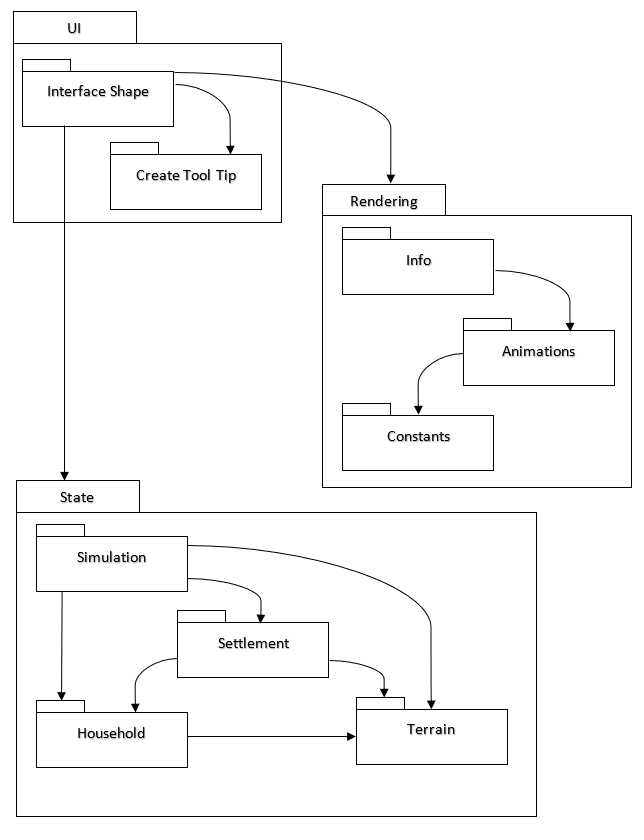
\includegraphics[width=10cm]{ArchitectureDiagram}
		\caption{Architecture diagram for the system, showing how the UI checks the state of the simulation and passes this to be rendered.}
		\label{fig:Architecture}
		\end{figure}
	
		\subsection{Changes}
			A number of changes in the implementation were made, some due to what seemed to be implementation errors in the original code and others due to functionality not making sense with what was trying to be achieved. Those which affect functionality have been implemented as explained, however when the Legacy Mode setting is enabled, these changes are reverted back to how they were in the original implementation.
				\subsubsection{Death Due to Lack of Grain}
				In the original NetLogo code, if a household did not have enough grain to survive a year then a single person would die and the grain would be set to zero. In reality this doesn't make sense, as if a household has no food, then no one would survive. The reimplementation changed this so that only the family members who can be fed will survive.\\
				\subsubsection{Population Increases}
				In the original code, if the total current population is less than or equal to the historical projected population then the population can increase. At first glance this seems to be correct, however this allows the population to always grow slightly faster than the projected historical value, and thus in the reimplementation this is changed so that the population will only increase if it is less than the historical projected population.\\
				\subsubsection{Generational Changes in Ambition and Competency}
				In the original code, if the ambition or competency for a household moved out of the bounds set (minimum, up to 1) then a new value would be generated until it fell within the bounds. This means that the computational time for the ambition and competency changes are unbounded. In the reimplementation, a value within the possible range is generated.\\
				\subsubsection{Order of Field Claimants}
				In the original code, households claimed fields in ascending order of how much grain they currently have. This seemed inconsistent with every other operation being independant of grain or ordering, in the reimplementation, this ordering is randomised each year.
	\section{Test Cases}

	\section{Conclusions}
		The application as designed seems to run much faster than its predecessor, while also being written in a more extensible manner. For clients, there are quality of life features that were implemented which were not in the original, for example being able to set up multiple runs of the same settings to automatically continue as well as being able to easily save graphs which are generated. In the original, a single graph could be saved at a time. In the reimplementation, all graphs could be saved at once, or a graph could be zoomed in on before being saved.
	\begin{thebibliography}{9}
		
	\end{thebibliography}

	\appendix
	\section{Manual}
		\subsection{Sliders}
			The left hand side of the interface contains a set of sliders which may be adjusted to give different parameters to the program. On adjustment, the sliders automatically reset the simulation with the changed values. Below sliders are check boxes, which function similarly - resetting the simulation on being changed. One check box asks the users for a seed and then passes this to the simulation.
		
		\subsection{Simulation display}
			The central portion of the interface displays the current state of the simulation, in which the user may right click any block to see a description of the current parameters associated with that block. To clear the display of information when no longer required, the user may left click. The information displayed depends on what type of block was clicked on, as follows:
			\subsubsection{Settlement}
				Settlements are represented by houses, where the size of the house represents the total population of the settlement.\\
				When right clicked on, settlements display their total population, and how many households are contained within.\\
			\subsubsection{Fields}
				Fields are represented by a circle (unharvested) or a piece of barley. The colour of the symbol is related to the colour of the household which has claimed the field, with purple representing the top 33\% of wealth, blue representing the middle 33\% and yellow representing the bottom 33\%.\\
				When right clicked on, fields will display whether or not they have been harvested, their fertility, their potential harvest for the year and the number of years it has been since the field has been harvested.\\
			\subsubsection{Land}
				The shade of green of each of the block of represents its fertility, where a darker colour means that it is more fertile. Right clicking on a piece of land displays its fertility and what its potential harvest would be if it were to be claimed and harvested.
				
		\subsection{Graphs of data}
			Two displays are available on the right hand side of the interface. Each is controlled by a drop down box beneath it which when clicked allows the user to choose one of the eleven graphs to be displayed. There is also a tool bar underneath each graph which allows the user to interact with the graph through actions such as panning or zooming. To save an individual graph one may click the save button in the toolbar. To save all the graphs into a folder of your choosing, click “Save all figures” and enter the name of the folder. 
			
	\section{Technical API Manual}
		This section will assume a familiarity with how the simulation is meant to function as well as the code of Simulation, Settlement, Household and Terrain, although a brief description of their functionality will be described. If additional variables are required in Settlement, Household or Terrain, note that these variables must first be added to the "\_\_slots\_\_" list at the top of the class in order to be used. This is to provide speedup to accessing variables and reduce memory usage overall and is opposed to the usual python dictionary which is used to store variables within classes.
			\subsection{Simulation}
				The Simulation class forms a wrapped for all of the other simulation objects, holding data that is required globally throughout. It also controls some of the order of operations. For extensibility, the simulation class would probably not provide much help outside of changes to instantiation. If one were to want different households or settlements to run with different parameters, this is where one would make the changes.
			\subsection{Settlement}
				The Settlement class holds the households which exist in a specific area together, controls the removal of households when their population reaches 0 and ensures that the households within run their yearly simulations in a random order. If one were to want to change the order in which the simulation is run, or change behaviour of household removal, this is the file in which changes should be made.
			\subsection{Household}
				The Household class controls the year to year activities of individual houses, including farming, using food, population increases and changes to ambition and competency over generations. If one were to want to change any general behaviour of the individual households, this is likely to be the correct area to look. Due to how python treats functions, functions can be replaced in certain households without affecting how all households function. If this is done, it must be ensured that the population of the settlement and total population are adjusted when the population is adjusted, and that the grain of the household at the end of the year is added to the total grain.
			\subsection{Terrain}
				The Terrain class maintains information about the state of the land in a specific position, as well as containing information about what its position is. It is unlikely that extensibility would come from altering this class, but if it is necessary, then it must be ensured that the years not harvested is incremented each year, harvested is set to false at the start of the year, the fertility and harvest are set every year, and the claim and unclaim functions need to maintain their current functionality. 
	\section{Screenshots}
	\begin{figure}[!htb]
		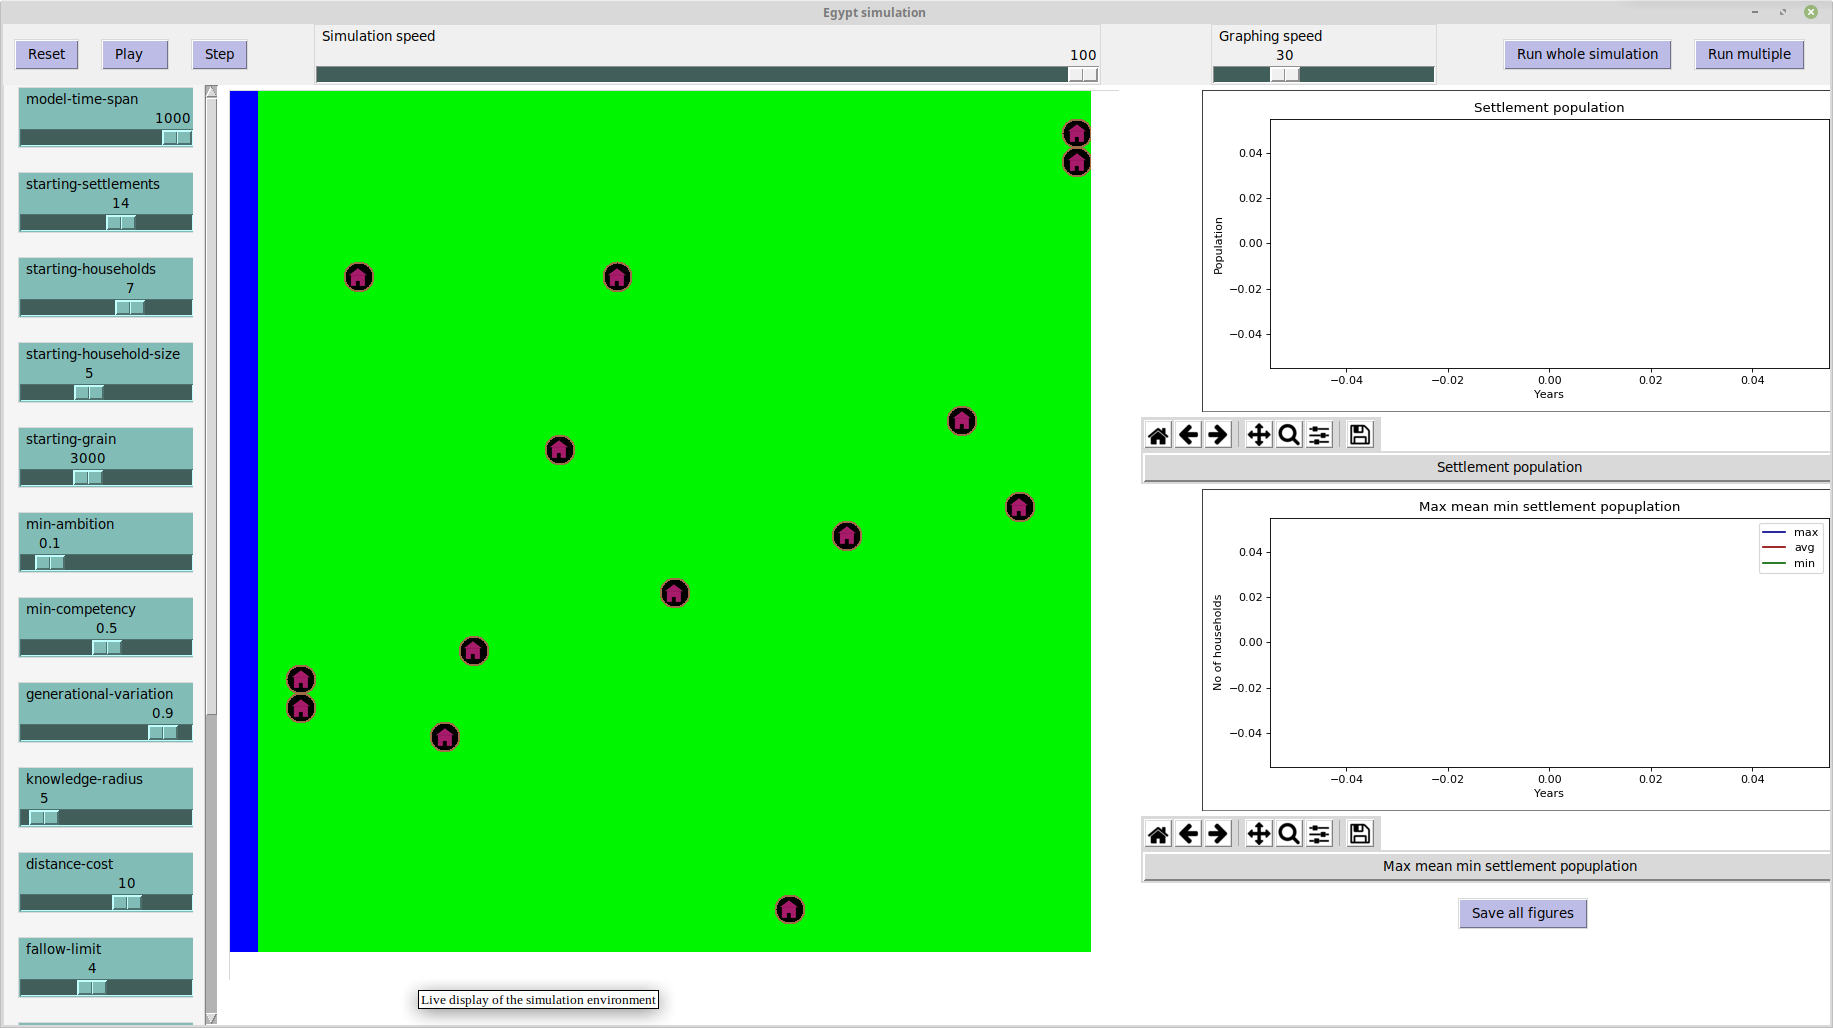
\includegraphics[width=15cm]{OnOpen}
		\caption{Screenshot of the application once opened, without any actions being performed.}
		\label{fig:OnOpen}
	\end{figure}
	
	\begin{figure}[!htb]
		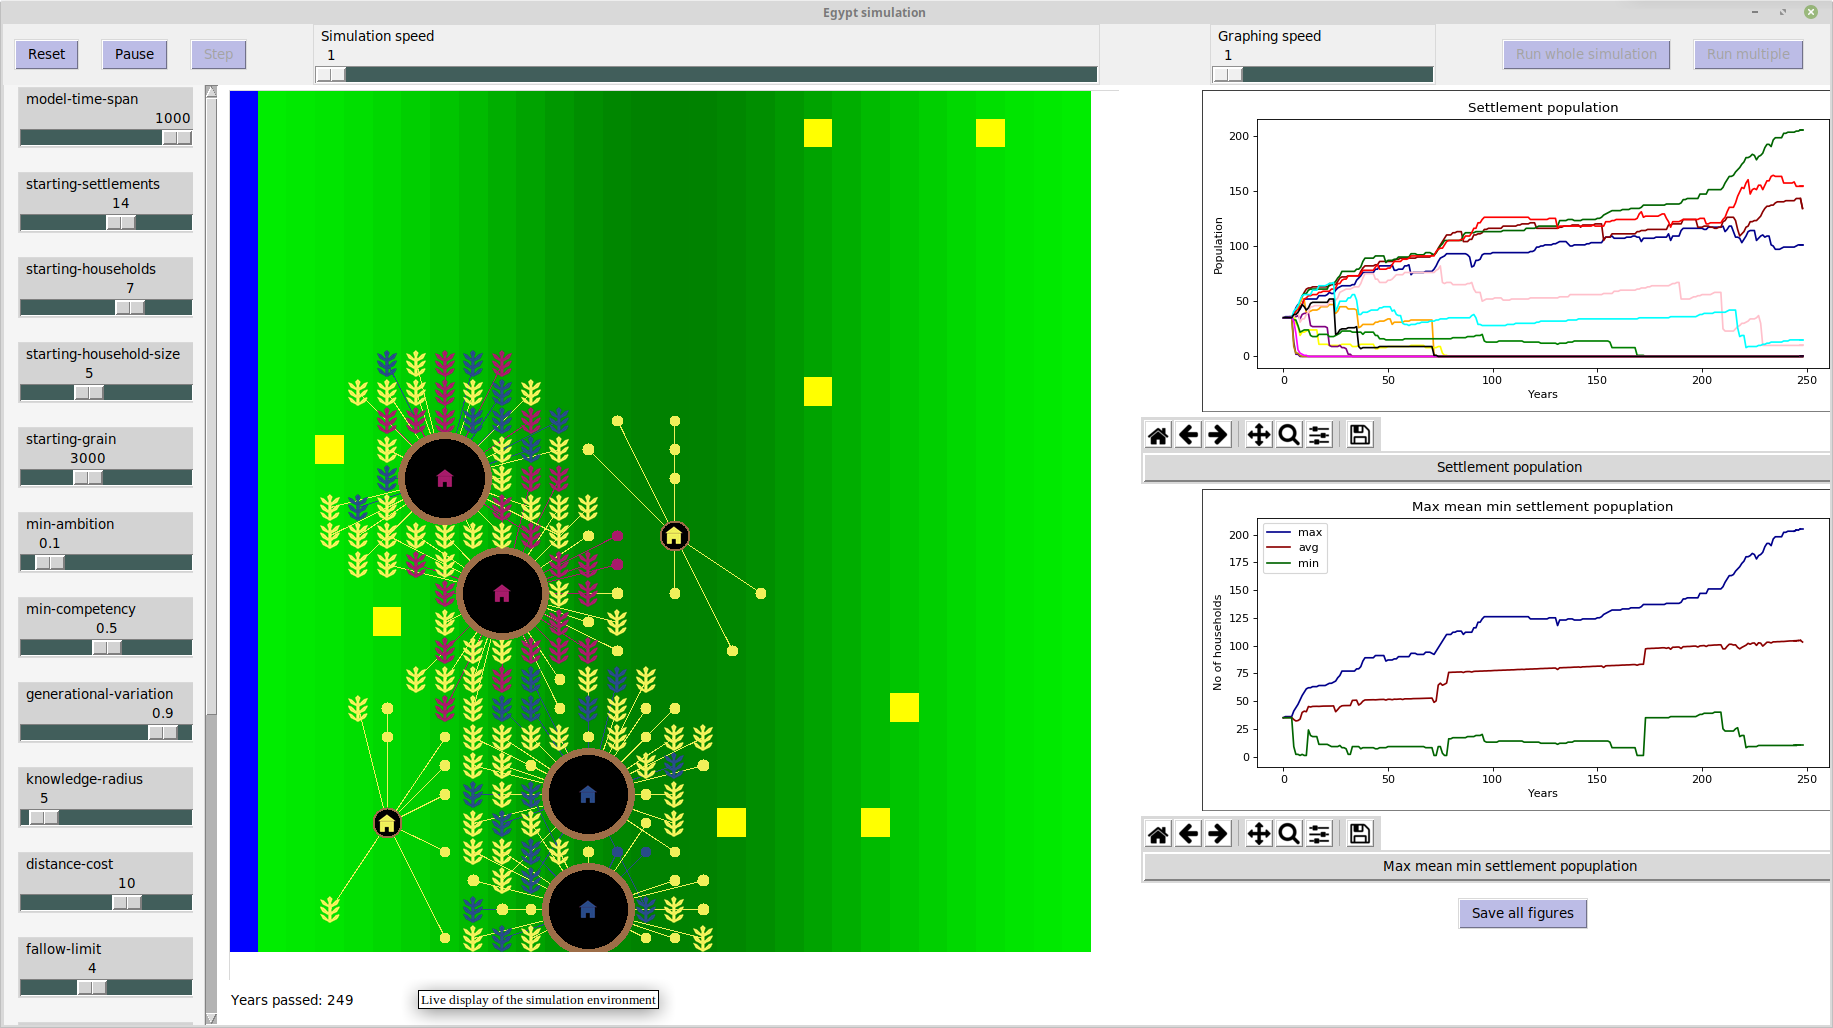
\includegraphics[width=15cm]{WhileRunning}
		\caption{Screenshot of the application once a run has begun, taken at a slow simulation speed to prevent screentearing during a screenshot.}
		\label{fig:WhileRunning}
	\end{figure}
	
	\begin{figure}[!htb]
		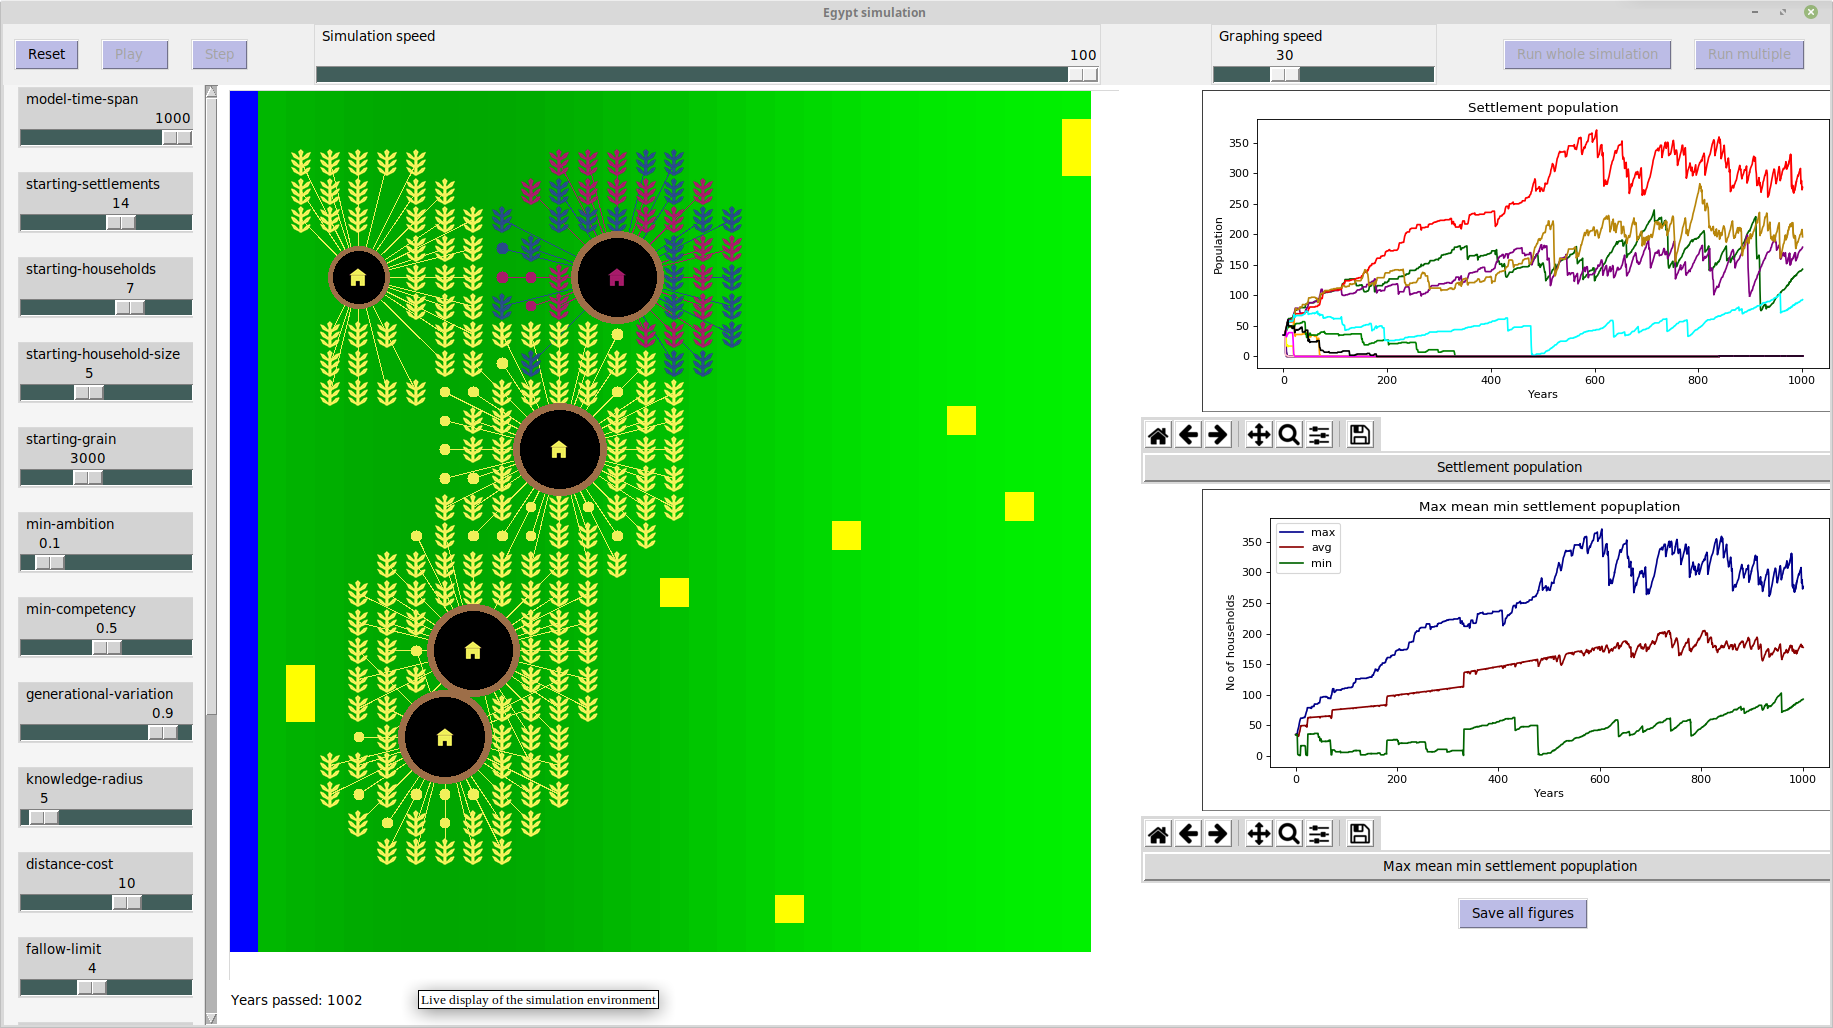
\includegraphics[width=15cm]{FinishedRunning}
		\caption{Screenshot of the application once a run has completed.}
		\label{fig:FinishedRunning}
	\end{figure}
	
	\begin{figure}[!htb]
		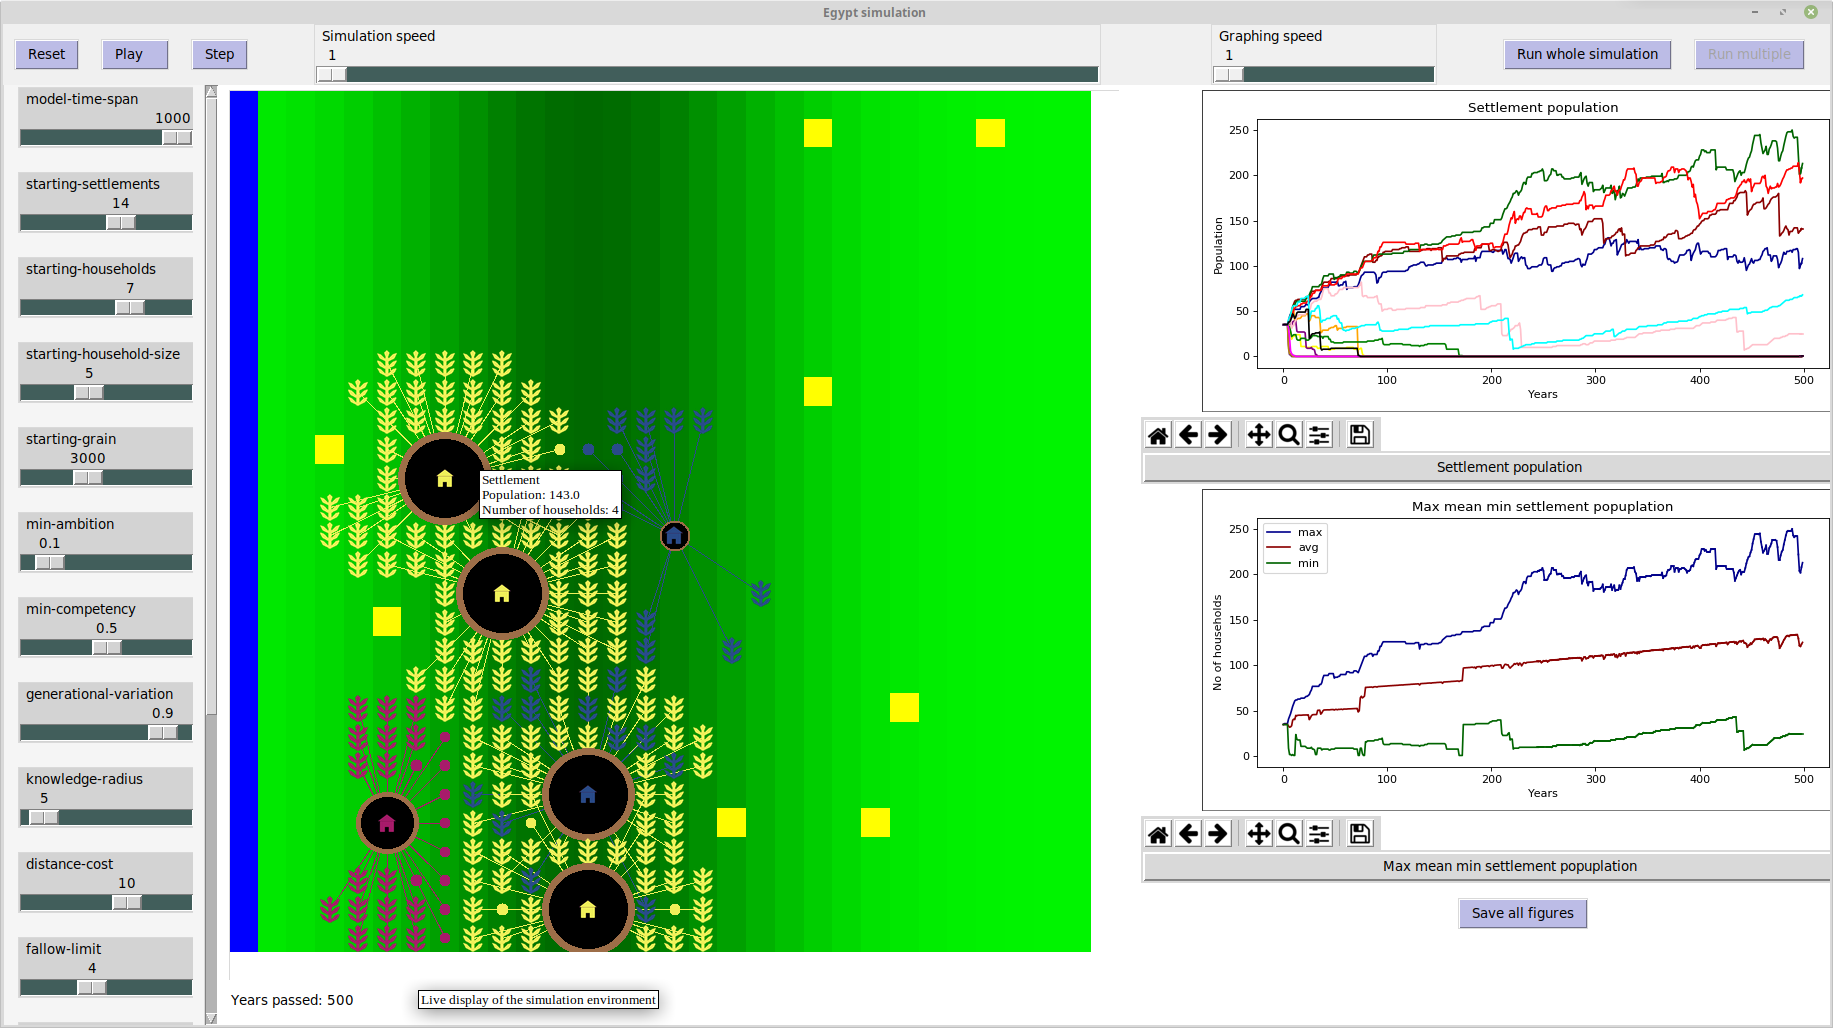
\includegraphics[width=15cm]{RightClickOnSettlement}
		\caption{Screenshot of the application during a run, with the simulation paused and the output of right clicking on a settlement shown.}
		\label{fig:ClickOnSettlement}
	\end{figure}
	
	\begin{figure}[!htb]
		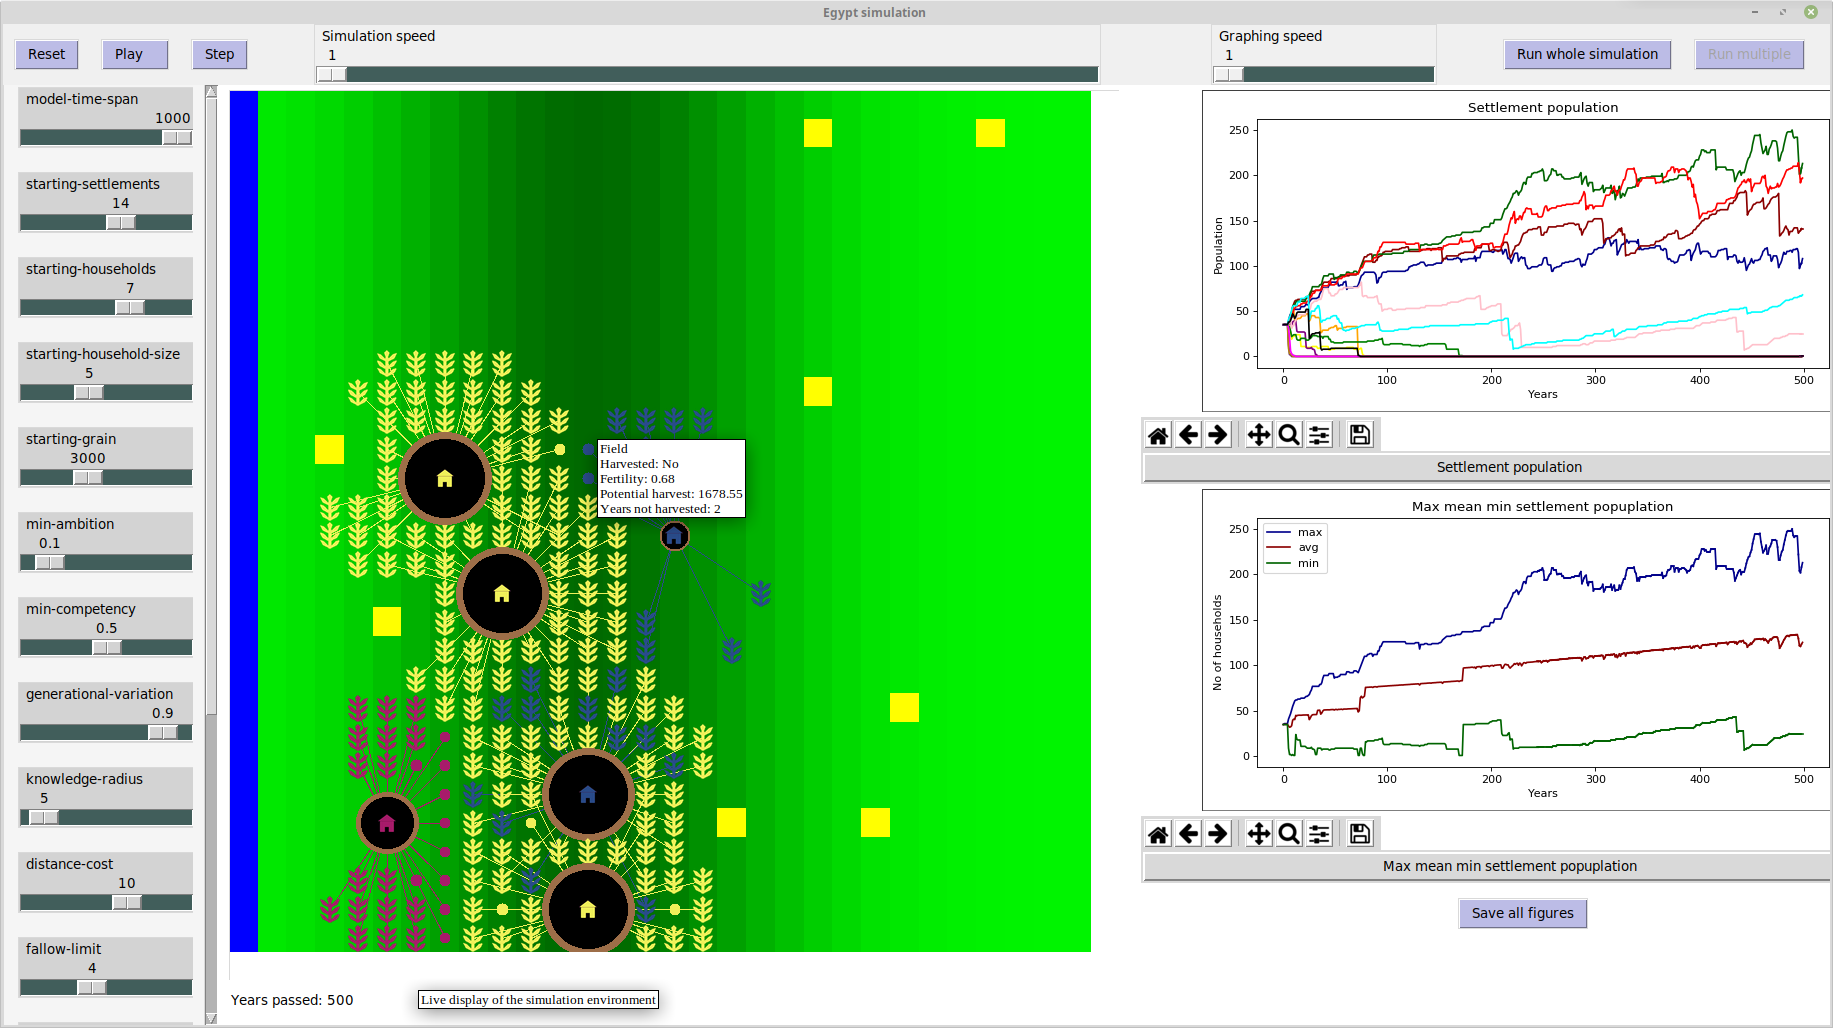
\includegraphics[width=15cm]{RightClickOnNotHarvestedField}
		\caption{Screenshot of the application during a run, with the simulation paused and the output of right clicking on an unharvested field shown.}
		\label{fig:ClickOnUnharvested}
	\end{figure}
	
	\begin{figure}[!htb]
		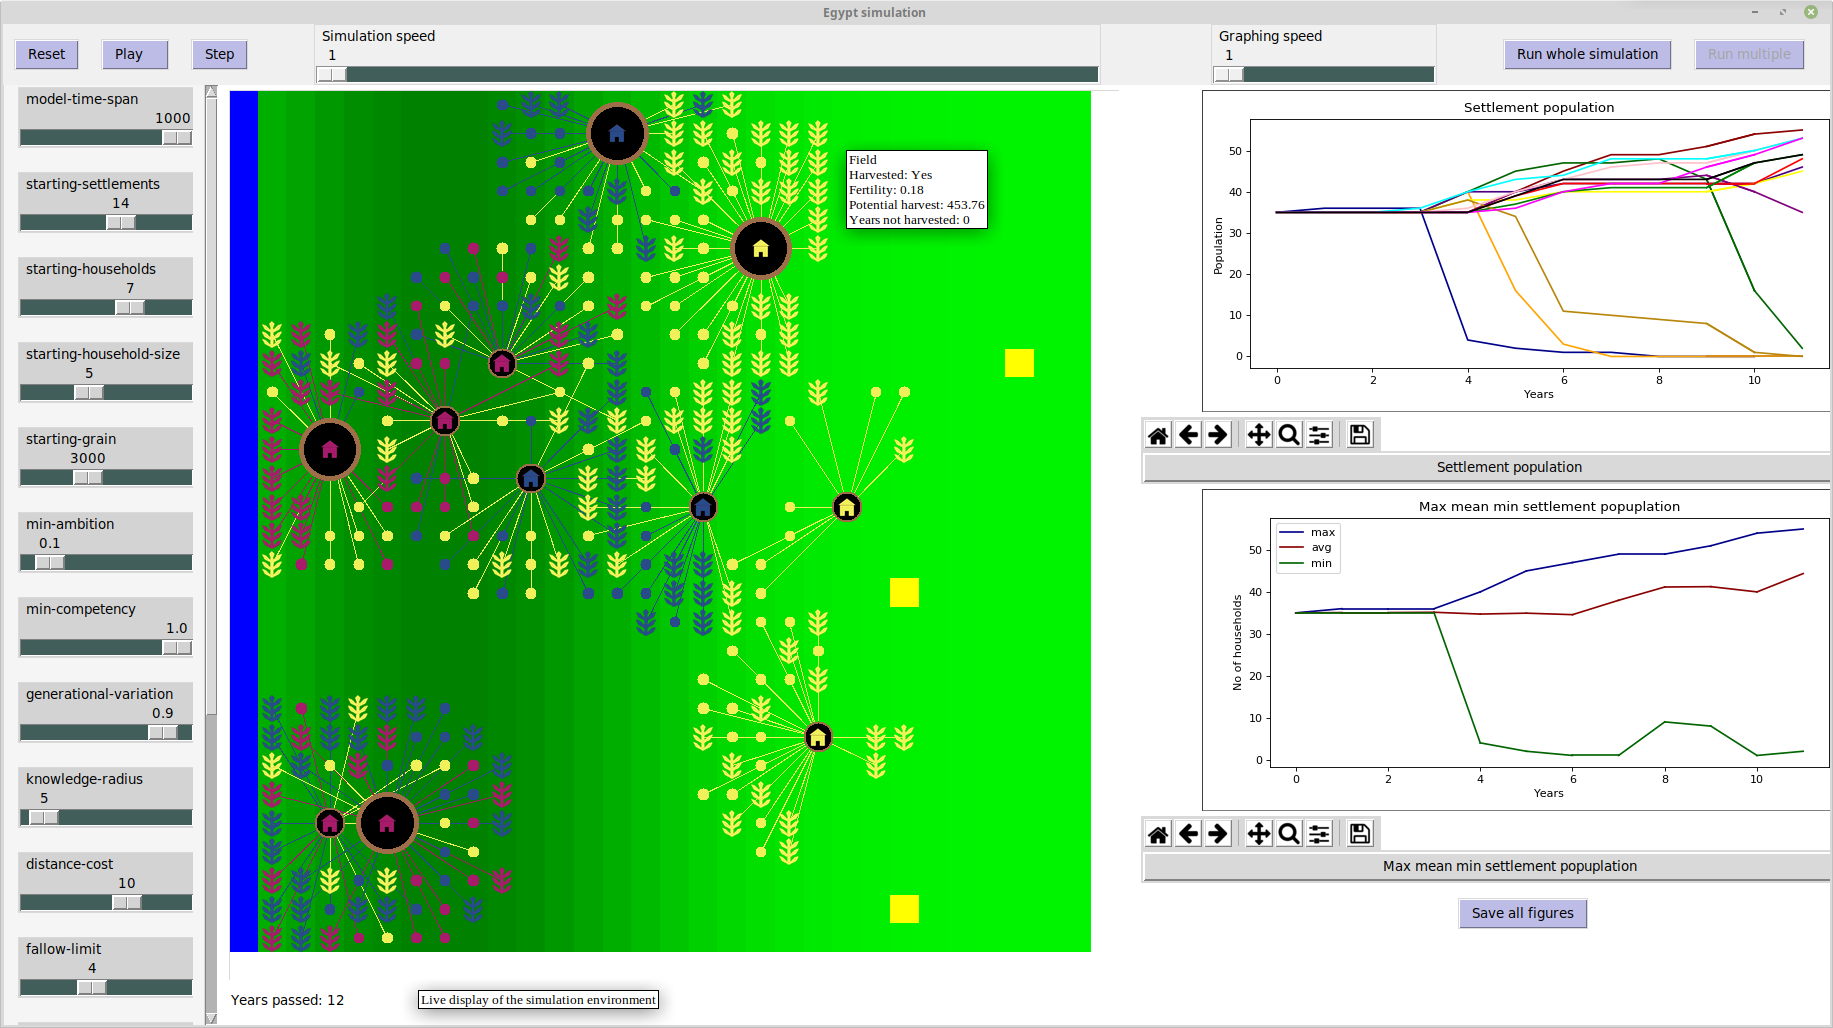
\includegraphics[width=15cm]{RightClickOnHarvestedField}
		\caption{Screenshot of the application during a run, with the simulation paused and the output of right clicking on a harvested field shown.}
		\label{fig:ClickOnHarvested}
	\end{figure}
	
	\begin{figure}[!htb]
		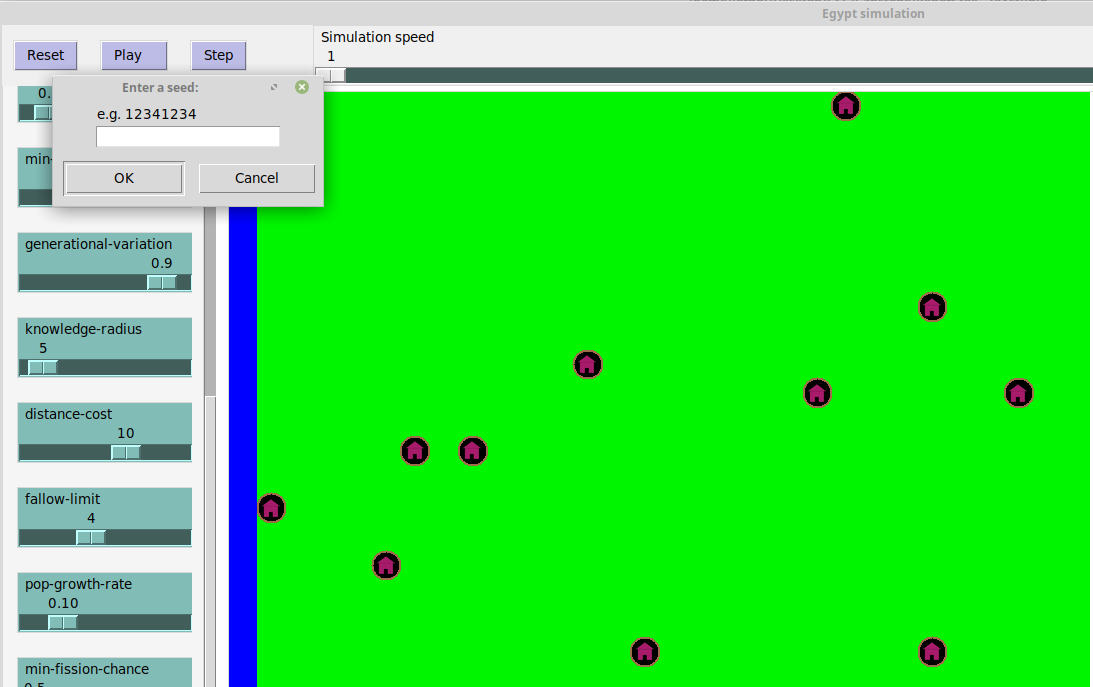
\includegraphics[width=15cm]{SeedEntry}
		\caption{Screenshot of the application showing how a manual seed is entered.}
		\label{fig:Seed Entry}
	\end{figure}
	
	\begin{figure}[!htb]
		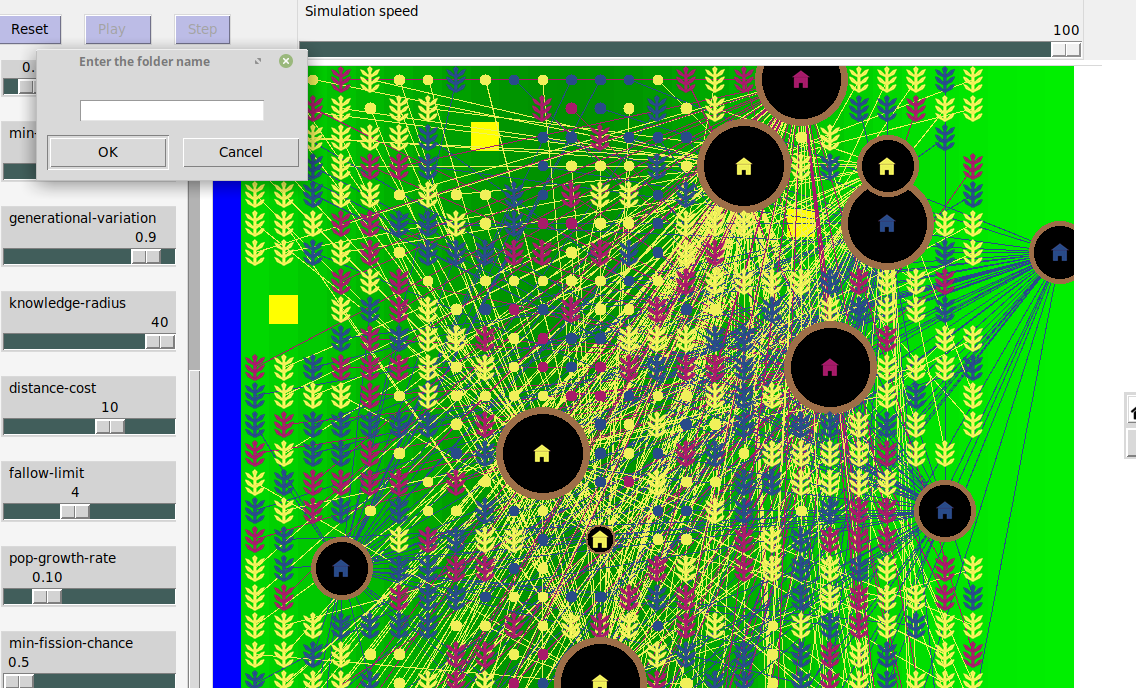
\includegraphics[width=15cm]{SaveAll1}
		\caption{Screenshot of the application showing the dialog asking for a foldername to save multiple figures in for the "Save all Figures" button.}
		\label{fig:SaveAllFolder}
	\end{figure}
	
	\begin{figure}[!htb]
		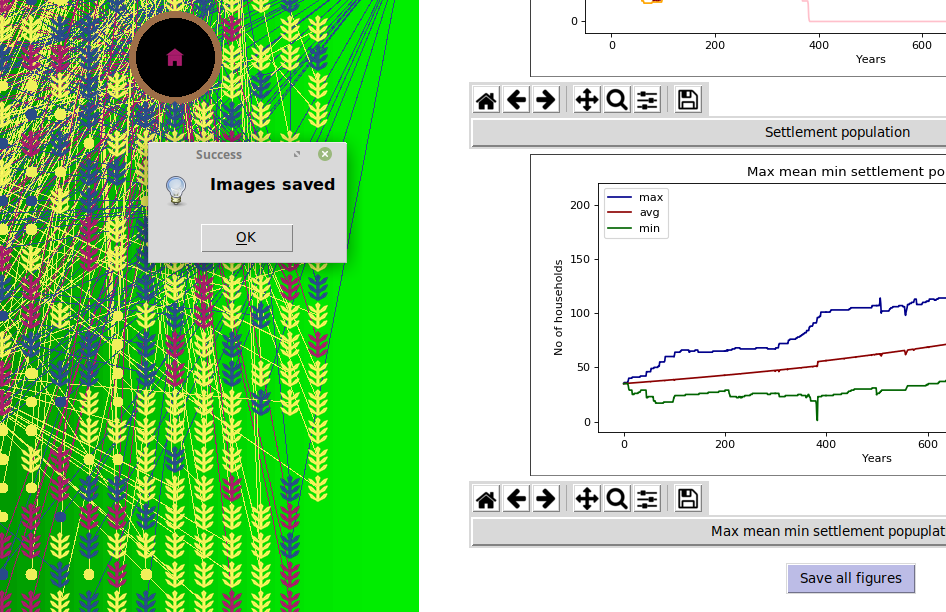
\includegraphics[width=15cm]{SaveAll2}
		\caption{Screenshot of the application showing output of the "Save all Figures" button once all figures have been saved.}
		\label{fig:SaveAllSaved}
	\end{figure}
\end{document}